\begin{exmp}
\label{motivatingExample}
To illustrate the impact of estimation delay $\sDelay$ and estimate inaccuracy $\sAccu$ on control performance, we show a simple PID controlling the motion of a decoupled point mass in the $(x,y)$ plane.
The position of the point mass must follow a reference constant trajectory, whose $x$ dimension is shown in Fig.~\ref{fig:toyplot} (the same plot can be obtained for the $y$ position).
We simulate three cases of estimation (and therefore actuation) delay and error, where a larger delay value $\sDelay$ implies a smaller estimation error $\sAccu$.
As can be noted in Fig.~\ref{fig:toyplot}, the effect of delay can be non-negligible.
Moreover, decreasing delay doesn't necessarily imply better tracking performance: the effect of the concomitant estimation error must be taken into account. 
In this example, it can be seen that the increasing error causes the tracking performance to worsen.
Running an estimation task with a fixed smaller delay but larger estimation error does not necessarily solve the problem of degraded performance, as can be seen in Fig.~\ref{fig:toyplot}.

Therefore, there is a need to rigorously quantify the trade-off between computation time and estimation error, then exploit that trade-off to achieve the best control performance under the problem constraints.
Rather than always run the estimation task to completion, it is useful to have several estimation tasks with varying utilities (i.e., varying delay/error trade-offs).
These can then be used at runtime to satisfy the control objectives.
\exmend

\begin{figure}[t]
\centering
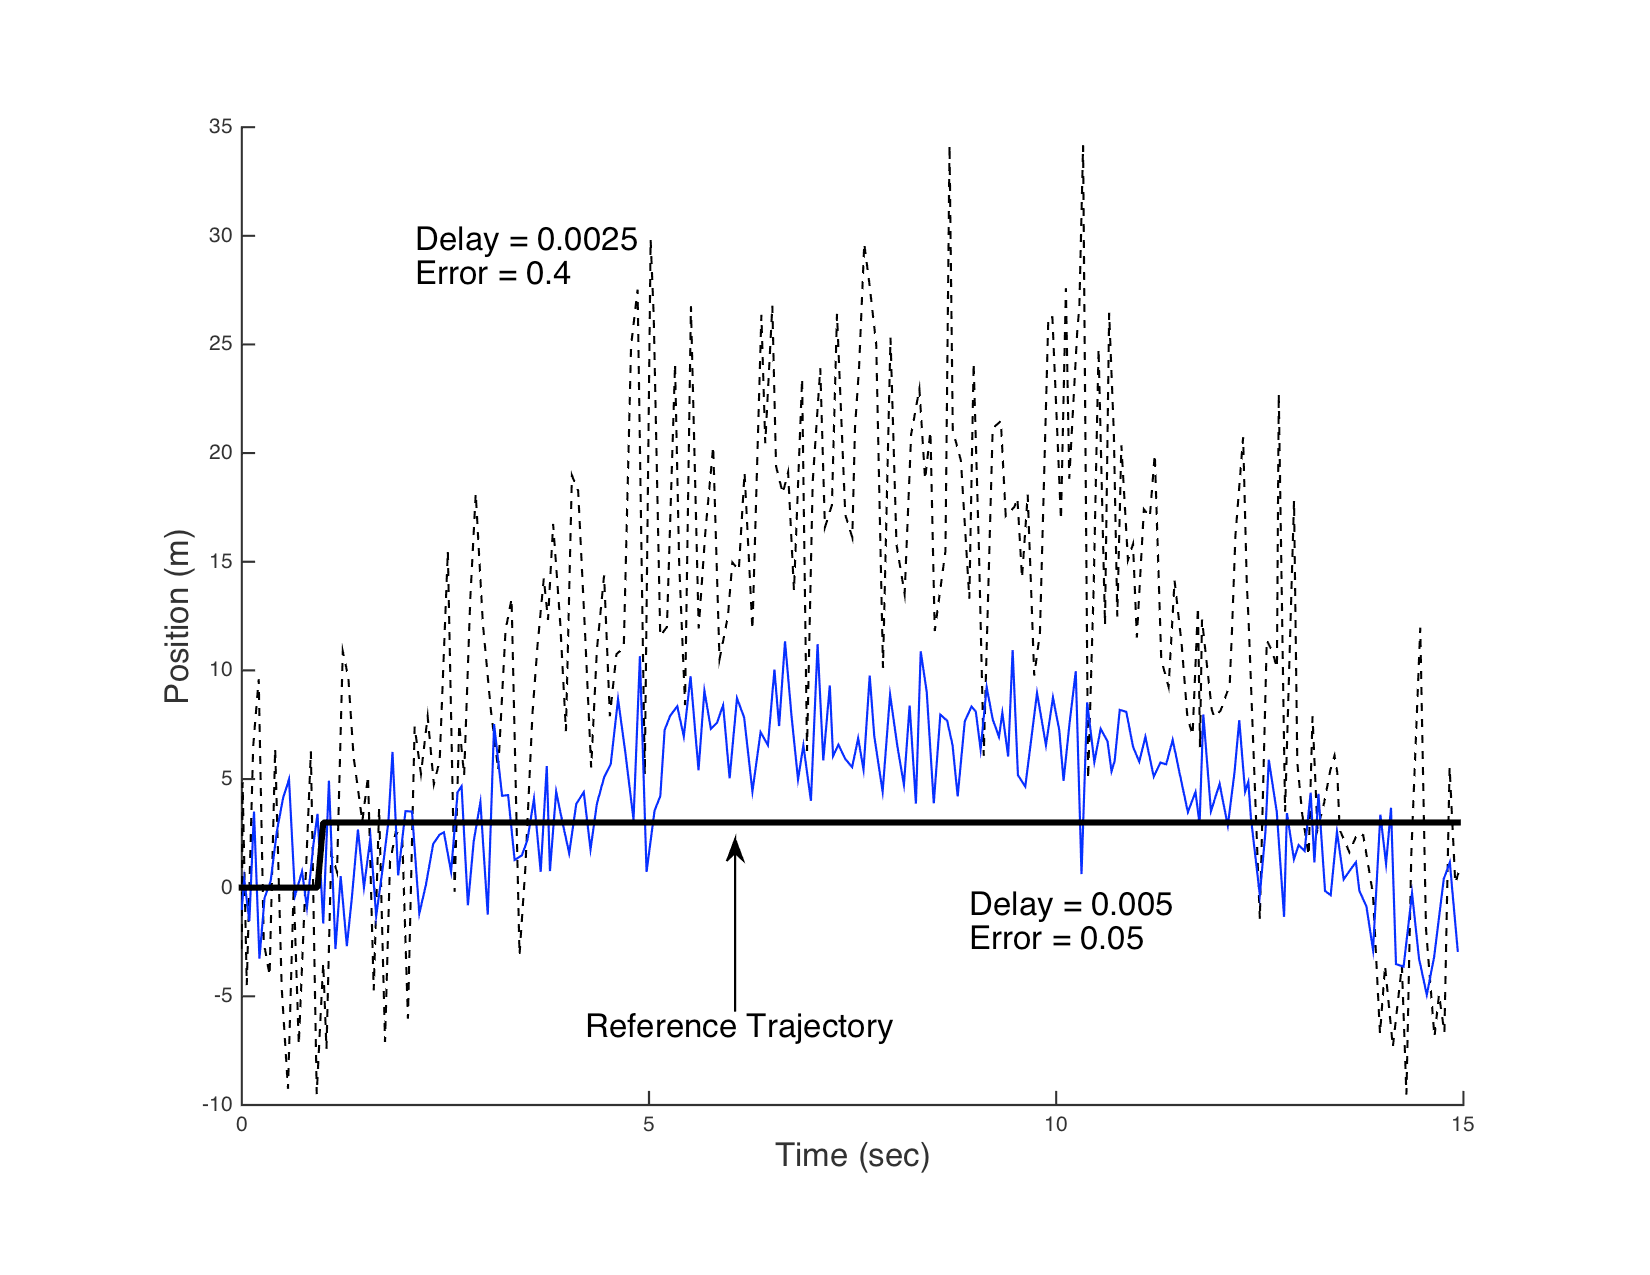
\includegraphics[scale=0.3]{figures/toyplot}
\caption{Effect of delay,error values on control performance.}
\label{fig:toyplot}
\end{figure}
\end{exmp}

